\documentclass[a4paper 10pt]{article}
\usepackage[english,polish]{babel}
\usepackage[MeX]{polski}
\usepackage[utf8]{inputenc}
\usepackage[T1]{fontenc}
\usepackage[letterpaper, portrait, margin=0.5in]{geometry}
\usepackage{graphicx}
\usepackage{listings}
\usepackage{subfigure}
\usepackage{dashrule}
\usepackage{listings}
\usepackage{float}
\usepackage{amsmath}
\usepackage{listings}
\usepackage{multirow}
\usepackage{amsmath}
\usepackage{xcolor}
\usepackage{listings}
\usepackage{hyperref}
\hypersetup{ hidelinks = true, } 
\lstset{
    frame=single,
    breaklines=true,
    postbreak=\raisebox{0ex}[0ex][0ex]{\ensuremath{\color{red}\hookrightarrow\space}}
}


\renewcommand{\rmdefault}{ptm}
  
\frenchspacing

% Used to add additional dot in enumerations
\usepackage{titlesec}
\titlelabel{\thetitle.\quad}
\title{\textbf{Techniki Optymalizacji} \\
Laboratorium nr 4 \\
Sprawozdanie}
\author{Paulina Sadowska, Rafał Araszkiewicz}
\begin{document}
\maketitle

\section{Wprowadzenie}
Celem ćwiczenia było dziesięciokrotne uruchomienie hybrydowego algorytmu ewolucyjnego z pełną elitarnością, uzyskanie danych statystyczny oraz wykresów kosztu ścieżki i czasu obliczania w poszczególnych generacjach algorytmu ewolucyjnego.

\section{Otrzymane wyniki}


\begin{figure} [H]
\centering
\caption{Czas wykonywania LS w kolejnych generacjach}
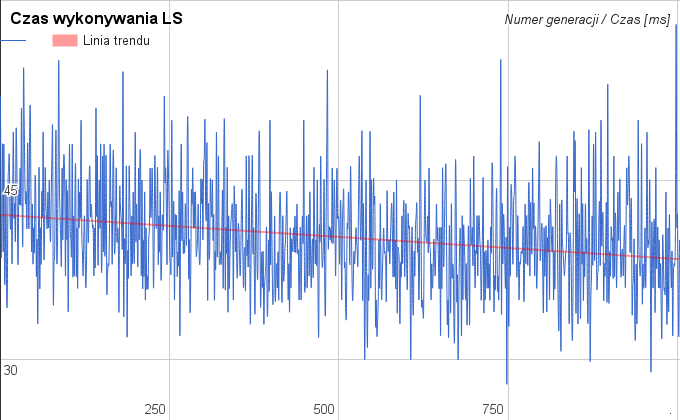
\includegraphics[angle=0,width = 1\textwidth, height=!]{images/czas_ls.png}
\label{Rys. Edges}
\end{figure}

\begin{figure} [H]
\centering
\caption{Koszt najlepszej ścieżki w kolejnych generacjach}
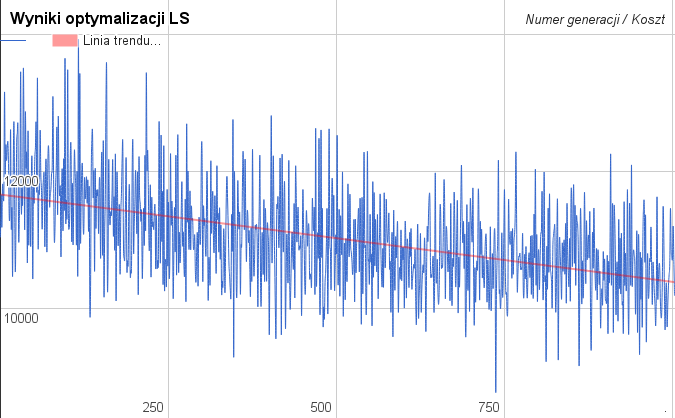
\includegraphics[angle=0,width = 1\textwidth, height=!]{images/wyniki_opti.png}
\label{Rys. Node}
\end{figure}


\begin{table}[H]
\centering
\caption{Statystyki otrzymane z 10 powtórzeń algorytmu ewolucyjnego oraz NNG + MSLS}
\label{my-label}
\begin{tabular}{|l|c|c|}
\hline
                    & \multicolumn{1}{l|}{\textbf{Evolutionary}} & \multicolumn{1}{l|}{\textbf{NNG + MSLS}} \\ \hline
\textbf{Best cost}  & 8771                                       & 9510                                     \\ \hline
\textbf{Mean cost}  & 9221                                       & 9525                                     \\ \hline
\textbf{Worst cost} & 9363                                       & 9664                                     \\ \hline
\textbf{Best time}  & 41.1s                                      & 36.4s                                    \\ \hline
\textbf{Mean  time} & 41.1s                                      & 41.1s                                    \\ \hline
\textbf{Worst time} & 41.1s                                      & 46.2s                                    \\ \hline
\end{tabular}
\end{table}

\end{document}
\\